\chapter{METODOLOGÍA}

\section{ENFOQUE Y DISEÑO DE LA INVESTIGACIÓN}
El presente trabajo de investigación se basa en un enfoque cuantitativo de tipo experimental computacional. Se implementa un simulador de la capa física del estándar IEEE 802.11bb en el lenguaje de programación Python, modelando de manera integrada las etapas de un sistema transmisor-receptor óptico y un canal de propagación inalámbrico para un enlace de tipo Vehículo a Infraestructura (V2I).

La arquitectura del simulador está estructurada de forma modular en bloques de procesamiento digital y analógico secuenciales. La integración funcional de estos bloques permite evaluar el comportamiento de la señal desde la generación de datos binarios hasta su reconstrucción final en el receptor. Para caracterizar el rendimiento de la comunicación bajo condiciones exteriores realistas expuestas al ruido solar y a la atenuación meteorológica, se utiliza la simulación estocástica por el método de Monte Carlo, estimando de forma empírica la Tasa de Error de Bit (BER) y la velocidad de transmisión efectiva (\textit{Throughput}) en función del barrido de la distancia geométrica del enlace.


\section{ARQUITECTURA GENERAL DEL TRANSMISOR Y RECEPTOR LC (IEEE 802.11BB)}
La arquitectura del sistema de comunicación implementado se basa en una estructura simétrica de procesamiento que sigue los lineamientos de la capa física (LC PHY). Las etapas del procesamiento de señal digital y analógica que componen el transmisor y el receptor de este simulador se ilustran detalladamente en el diagrama de bloques del transmisor (Fig. \ref{fig:transmisor_bloques}) y del receptor (Fig. \ref{fig:receptor_bloques}) descritos en el Capítulo 1, los cuales delimitan la integración funcional de todo el sistema.

\section{DISEÑO E IMPLEMENTACIÓN DEL TRANSMISOR (TX) ÓPTICO}
Para materializar la arquitectura de la capa física del estándar IEEE 802.11bb, se realiza una implementación modular en el lenguaje de programación Python. En esta sección se describe la estructura del bloque transmisor (Tx) óptico y su relación directa con el procesamiento en el bloque receptor (Rx). En la Tabla \ref{tab:bloques} se presenta la correspondencia detallada entre cada uno de los bloques lógicos definidos por la normativa y las funciones de software desarrolladas para la simulación. Como se observa en dicha tabla, para cada etapa de procesamiento de la señal en el transmisor se programa una función específica en la biblioteca \texttt{physical\_layer.py}. De igual manera, se muestra la correspondencia con las funciones receptoras equivalentes, las cuales están encargadas de realizar el procesamiento inverso para recuperar la información transmitida. A continuación, se detallan los principios de diseño y la lógica de implementación de cada uno de los módulos que conforman el transmisor óptico, presentados en el orden secuencial de la cadena de transmisión.


\begin{table}[H]
\centering
\caption{Correspondencia de Bloques del Estándar IEEE 802.11bb a la Implementación del Transmisor y Receptor}
\label{tab:bloques}
\begin{tabular}{|p{4.5cm}|p{4.8cm}|p{5cm}|}
\hline
\textbf{Bloque IEEE 802.11bb} & \textbf{Función en TX (Python)} & \textbf{Función en RX (Python)} \\ \hline
FEC Encoder (Tasa 1/2) & \texttt{fec\_encoder()} & \texttt{fec\_decoder()} (Viterbi con Erasures) \\ \hline
Puncturing & \texttt{puncture()} (Tasas 2/3, 3/4, 5/6) & \texttt{depuncture()} (Inserción de Erasures) \\ \hline
Interleaving \& Mapping & \texttt{interleave()} / \texttt{constellation\_mapping()} & \texttt{deinterleave()} / \texttt{constellation\_demapping()} \\ \hline
IDFT / DFT & \texttt{idft\_processing()} (\texttt{np.fft.ifft}) & \texttt{dft\_processing()} (\texttt{np.fft.fft}) \\ \hline
Insert / Remove GI & \texttt{insert\_guard\_interval()} & \texttt{remove\_guard\_interval()} \\ \hline
Windowing & \texttt{windowing()} (Coseno Alzado) & Sin equivalente directo \\ \hline
I/Q Mod / Demod & \texttt{iq\_modulation()} & \texttt{iq\_demodulation()} (Filtro Butterworth) \\ \hline
DC bias / DC block & \texttt{add\_dc\_bias()} (Adaptativo) & \texttt{remove\_dc\_bias()} (Mean Removal) \\ \hline
TX OFE / RX OFE & \texttt{tx\_optical\_front\_end()} (Clipping LED) & \texttt{rx\_optical\_front\_end()} (Responsividad R) \\ \hline
FEQ & Sin equivalente directo & Ecualización de un toque (Single-Tap FEQ) \\ \hline
\end{tabular}
\end{table}

\subsection{FEC ENCODER (CODIFICADOR DE CANAL)}
El bloque FEC (\textit{Forward Error Correction}) introduce redundancia estructural y controlada en la secuencia de bits de entrada mediante un codificador convolucional implementado en la función \texttt{fec\_encoder()}. Esta etapa utiliza una tasa de codificación convolucional base $R_c = 1/2$ y una longitud de restricción $K = 3$. Los polinomios generadores del codificador en formato octal se definen como $G_0 = 7$ ($111$ en binario) y $G_1 = 5$ ($101$ en binario), lo que permite que por cada bit de información de entrada se generen dos bits codificados de salida, duplicando el flujo de datos. Cabe recalcar que, aunque el estándar IEEE 802.11 define una longitud de restricción $K=7$ para su codificador convolucional legado, en este trabajo se opta por una longitud de restricción simplificada de $K=3$ con fines de viabilidad computacional. Esto reduce los estados de trellis de $64$ a $4$ en la decodificación de Viterbi, disminuyendo los tiempos de simulación en Python por un factor de 16 sin alterar los principios de modelado de la corrección de errores ni la estructura de las máquinas de punzado.

\textbf{Entrada:} vector de bits de información de longitud $N_{\text{bits}}$. \textbf{Salida:} vector de bits codificados de longitud $2 N_{\text{bits}}$ (tasa base $1/2$), que pasa directamente al bloque de punzado.

\subsection{PUNCTURING (BLOQUE DE PUNZADO)}
Para lograr las tasas de codificación más altas especificadas en el estándar (como $2/3$, $3/4$ y $5/6$ necesarias para los esquemas MCS avanzados), se implementa la función \texttt{puncture()}. Este bloque remueve periódicamente bits específicos del flujo codificado de tasa 1/2 de acuerdo con patrones de máscara de punzado. En el extremo receptor, la función \texttt{depuncture()} realiza la operación inversa, reinsertando bits neutros (llamados borrados o \textit{erasures}) en las posiciones punzadas. Esta estructura de borrado es procesada por el algoritmo de decodificación de Viterbi, el cual omite el cálculo de la distancia de Hamming para dichos bits neutros, preservando la ganancia de codificación sin alterar la estructura del trellis.

\textbf{Entrada:} vector de bits codificados de tasa $1/2$. \textbf{Salida:} vector de bits punzados de tasa $R_c \in \{1/2, 2/3, 3/4, 5/6\}$ según el MCS activo, que pasa al entrelazador.

\subsection{BLOCK INTERLEAVER (ENTRELAZADOR)}
El bloque entrelazador reordena secuencialmente los bits provenientes del codificador convolucional mediante la función \texttt{interleave()}. El proceso aplica una técnica de entrelazado por bloques donde los bits se escriben fila por fila en una matriz bidimensional de 16 columnas y se leen columna por columna para formar un stream de salida unidimensional. Si el tamaño de la secuencia codificada no es un múltiplo exacto de 16 columnas, la función realiza un relleno automático (\textit{padding}) con ceros lógicos. Este bloque tiene como objetivo dispersar espacialmente los errores en ráfaga (\textit{burst errors}) que se producen en el canal óptico debido a desvanecimientos rápidos o sombras angulares, convirtiéndolos en errores aislados que pueden ser eficientemente resueltos por el decodificador FEC.

\textbf{Entrada:} vector de bits punzados. \textbf{Salida:} vector de bits entrelazados de la misma longitud, listo para la asignación de constelación.

\subsection{CONSTELLATION MAPPING (ASIGNACIÓN DE CONSTELACIONES)}
La secuencia de bits entrelazada se agrupa y asigna a símbolos complejos en el plano de fase mediante la función \texttt{constellation\_mapping()}. Esta función implementa la asignación por codificación Gray para asegurar que dos puntos adyacentes de la constelación difieran únicamente en un solo bit, minimizando la tasa de error por símbolo. El transmisor y receptor LC desarrollado soporta los seis esquemas de modulación multinivel definidos en el estándar IEEE 802.11bb: BPSK, QPSK, 16-QAM, 64-QAM, 256-QAM y 1024-QAM, cuyos factores de normalización de energía $K_{\text{norm}}$ se detallan en la Tabla~\ref{tab:mcs_velocidades_bb} del Capítulo~1.

\textbf{Entrada:} vector de bits entrelazados. \textbf{Salida:} vector de símbolos complejos QAM normalizados por $K_{\text{norm}}$ (Ec.~\ref{eq:k_norm}), con varianza unitaria. La salida ingresa directamente a la etapa de simetría hermitiana.

\subsection{HERMITIAN SYMMETRY (SIMETRÍA HERMITIANA)}
Para garantizar que la señal modulada multiportadora OFDM sea estrictamente real en el dominio del tiempo y sea compatible con la modulación de intensidad analógica del diodo LED, los símbolos complejos se organizan en el dominio de la frecuencia mediante la función \texttt{apply\_hermitian\_symmetry()}, aplicando la propiedad de simetría hermitiana descrita en la ecuación (\ref{eq:simetria_hermitiana_theory}) del Capítulo~1.

\textbf{Entrada:} vector de 234 símbolos QAM complejos normalizados. \textbf{Operación:} la función construye un vector espectral de 1024 puntos: coloca los 234 símbolos en los índices positivos (139--255 y 257--373), sus conjugados en los índices espejo, y ceros en las subportadoras de guarda, DC ($k=0$) y Nyquist ($k=512$). \textbf{Salida:} vector espectral hermitiano de $N_{\text{fft}} = 1024$ puntos listo para la IFFT.

\subsection{IDFT/IFFT (PROCESAMIENTO DE TRANSFORMADA INVERSA)}
El bloque IDFT traslada la señal desde el dominio de la frecuencia al dominio del tiempo. En la práctica, se implementa mediante el algoritmo de la IFFT a lo largo de las filas de la matriz en la función \texttt{idft\_processing()}, calculada de acuerdo con la ecuación (\ref{eq:idft_sym}) del Capítulo~1 con un tamaño de FFT $N_{\text{fft}} = 1024$. La función realiza una comprobación estricta de la componente imaginaria residual, asegurando que la amplitud máxima de la componente compleja imaginaria resultante sea de valor despreciable (menor a $10^{-12}$) y extrayendo de forma limpia la parte real de la señal temporal.

\textbf{Entrada:} vector espectral hermitiano de 1024 puntos. \textbf{Salida:} vector temporal real de $N_{\text{fft}} = 1024$ muestras flotantes por símbolo (duración $12.8~\mu$s). La salida pasa directamente a la inserción del prefijo cíclico.

\subsection{GUARD INTERVAL INSERTION (INSERCIÓN DE PREFIJO CÍCLICO)}
El bloque de prefijo cíclico, programado en \texttt{insert\_guard\_interval()}, copia las últimas muestras ($N_{\text{CP}}$ muestras) de cada símbolo OFDM de salida y las anexa al inicio del mismo, siguiendo la ecuación (\ref{eq:cp_insert}) del Capítulo~1.

\textbf{Entrada:} vector temporal real de 1024 muestras por símbolo. \textbf{Salida:} vector extendido de $N_{\text{fft}} + N_{\text{CP}}$ muestras, con los tres modos implementados:
\begin{itemize}
\item \textbf{GI de 0.8~µs:} $N_{\text{CP}} = 64$ muestras ($T_{\text{symbol}} = 13.6\ \mu\text{s}$).
\item \textbf{GI de 1.6~µs:} $N_{\text{CP}} = 128$ muestras ($T_{\text{symbol}} = 14.4\ \mu\text{s}$).
\item \textbf{GI de 3.2~µs:} $N_{\text{CP}} = 256$ muestras ($T_{\text{symbol}} = 16.0\ \mu\text{s}$).
\end{itemize}
La salida pasa directamente al bloque de ventaneado.

\subsection{WINDOWING (VENTANEADO DE SÍMBOLOS)}
Para reducir las altas emisiones fuera de banda causadas por las discontinuidades abruptas en los flancos de subida y bajada entre símbolos OFDM consecutivos, se implementa el bloque de ventaneado en la función \texttt{windowing()}, implementando la ecuación (\ref{eq:windowing}) del Capítulo~1.

\textbf{Entrada:} vector OFDM con prefijo cíclico de $N_{\text{fft}} + N_{\text{CP}}$ muestras. \textbf{Operación:} se aplica una función de ventana de coseno alzado (\textit{Raised Cosine}) en las regiones de transición del símbolo con un factor de roll-off de 0.05. \textbf{Salida:} símbolo OFDM ventaneado con potencia espectral confinada dentro del canal de 20~MHz. La salida pasa a la modulación I/Q.

\subsection{I/Q MODULATION (MODULACIÓN I/Q)}
En los sistemas VLC para exteriores, las fuentes de iluminación artificial y las fluctuaciones eléctricas introducen un fuerte ruido ambiental y armónicos concentrados en las bajas frecuencias (por debajo de 2~MHz). Para eludir esta banda interferida, el transmisor implementa un bloque de conversión hacia arriba (\textit{up-conversion}) en la función \texttt{iq\_modulation()}, de acuerdo con la ecuación (\ref{eq:sf_if}) del Capítulo~1.

\textbf{Entrada:} vector temporal OFDM ventaneado (real, en banda base). \textbf{Operación:} multiplicación muestra a muestra por $\cos(2\pi f_{\text{IF}} t)$ con $f_{\text{IF}} = 20\text{ MHz}$ y $f_s = 80\text{ MHz}$. \textbf{Salida:} señal OFDM a frecuencia intermedia en la banda 10--30~MHz, como se ilustra en la Figura~\ref{fig:modulo_espectro_fi}. La señal resultante entra al bloque de bias DC.

\begin{figure}[H]
\centering
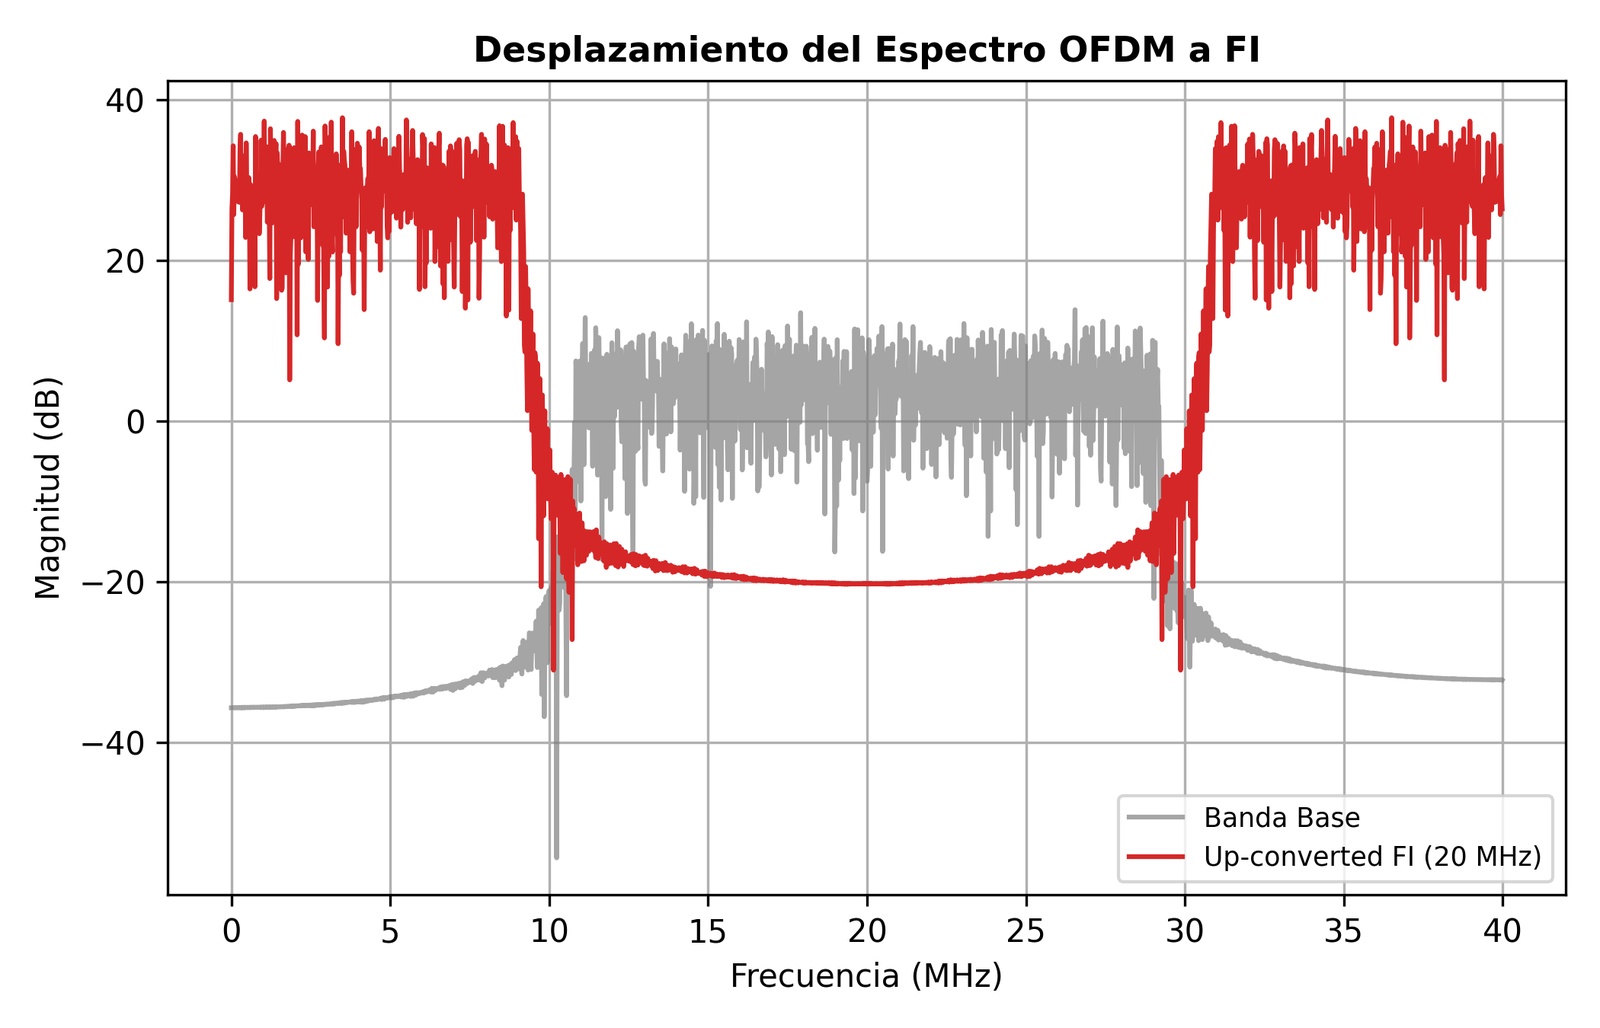
\includegraphics[width=0.75\textwidth]{modulo_espectro_fi.png}
\caption{Desplazamiento espectral de la señal multiportadora DCO-OFDM desde la banda base hacia la frecuencia intermedia de $20\text{ MHz}$ para eludir interferencias de bajas frecuencias.}
\label{fig:modulo_espectro_fi}
\end{figure}

\subsection{DC BIAS \& TX OFE (POLARIZACIÓN Y FRENTE ÓPTICO)}
Dado que los LEDs de iluminación vehicular se controlan por corriente eléctrica unidireccional y su potencia óptica de salida no puede adoptar valores negativos, la señal $s_{\text{IF}}(t)$ debe convertirse en una señal unipolar. El bloque DC bias, implementado en \texttt{add\_dc\_bias()}, añade un nivel de desplazamiento continuo constante $B_{\text{DC}}$ a la señal alterna, de acuerdo con la Ec.~(\ref{eq:dc_bias}) del Capítulo~1. La simulación utiliza un bias adaptativo: $B_{\text{DC}} = -\min(s_{\text{IF}}(t)) + 0.05$, que sitúa la señal justo sobre cero con un margen de $0.05\text{ A}$.

\textbf{Entrada:} señal OFDM alterna $s_{\text{IF}}(t)$ (bipolar). \textbf{Salida (DC Bias):} señal unipolar $s_{\text{biased}}(t)$ lista para el front-end óptico. Posteriormente, la señal unipolar ingresa al bloque del Frente Óptico de Transmisión (\texttt{tx\_optical\_front\_end()}), que aplica una función de recorte (\textit{clipping}) entre $led_{\text{min}} = 0.0\text{ A}$ y $led_{\text{max}} = 5.0\text{ A}$, y convierte la corriente en potencia óptica $P_{\text{opt}}(t)$ (Ec.~\ref{eq:p_opt_conv}). \textbf{Salida final:} potencia óptica instantanea en vatios, representada en la Figura~\ref{fig:modulo_led_intensidad}, que se propaga por el canal óptico.

\begin{figure}[H]
\centering
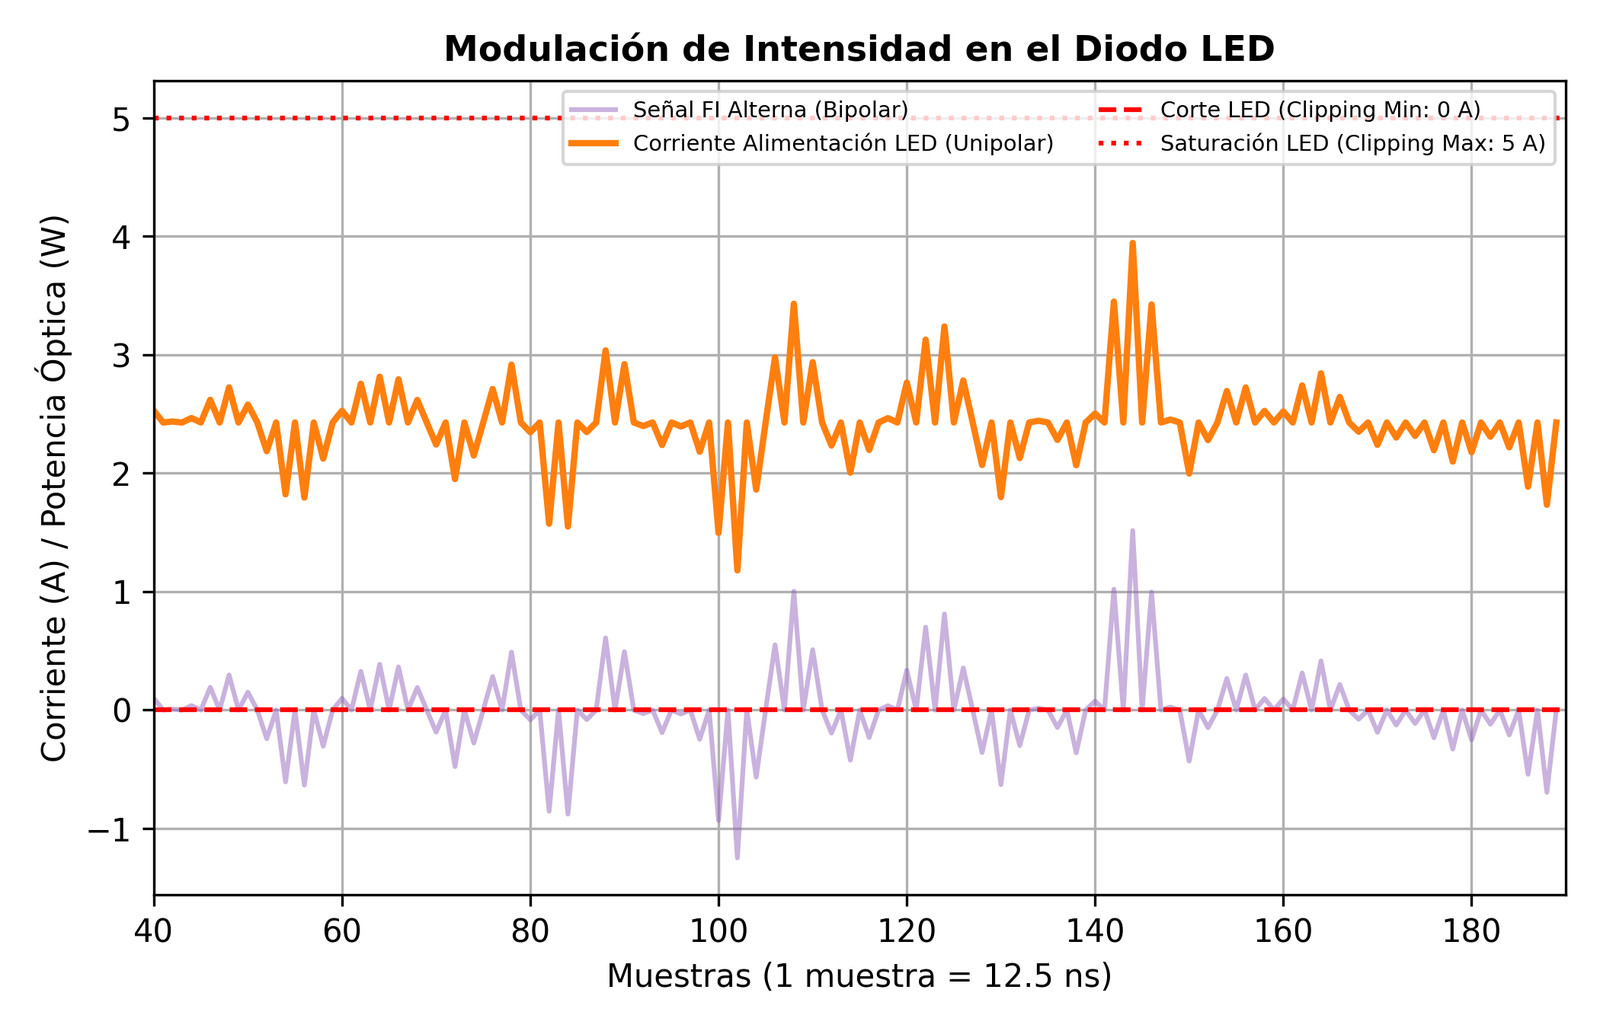
\includegraphics[width=0.75\textwidth]{modulo_led_intensidad.png}
\caption{Modulación de intensidad analógica en el emisor LED mostrando el desplazamiento mediante la componente de polarización continua ($B_{\text{DC}}$) adaptativa para operar en el rango unipolar.}
\label{fig:modulo_led_intensidad}
\end{figure}

\section{MODELO DE PROPAGACIÓN}

El canal óptico traduce la potencia óptica emitida por el LED vehicular en una señal eléctrica ruidosa en el fotodetector de la RSU, incorporando la atenuación geométrica, la extinción atmosférica y las fuentes de ruido propias de un entorno exterior V2I. En el simulador, toda esta lógica se centraliza en la función \texttt{optical\_wireless\_channel()} de la biblioteca \texttt{physical\_layer.py}. La Tabla~\ref{tab:funciones_canal} resume la correspondencia entre los bloques del canal y las funciones del código.

\begin{table}[H]
\centering
\caption{Correspondencia de bloques del canal óptico a funciones de la implementación}
\label{tab:funciones_canal}
\begin{tabular}{|p{5.2cm}|p{4.8cm}|p{4.2cm}|}
\hline
\textbf{Bloque del Canal} & \textbf{Función Python} & \textbf{Módulo} \\ \hline
Canal óptico vehicular completo & \texttt{optical\_wireless\_channel()} & \texttt{physical\_layer.py} \\ \hline
Parámetros geométricos y de escenario & \texttt{config\_entorno.py} & Configuración global \\ \hline
\end{tabular}
\end{table}

\subsection{FUNCIÓN \texttt{optical\_wireless\_channel()}}

Esta función implementa en cascada todos los fenómenos físicos del enlace V2I en un único bloque de procesamiento. El flujo interno sigue el orden: geometría del enlace $\rightarrow$ ganancia Lambertiana $\rightarrow$ atenuación atmosférica $\rightarrow$ cálculo de ruido $\rightarrow$ inyección de ruido $\rightarrow$ registro de SNR.

\textbf{Entradas:}
\begin{itemize}
    \item $P_{\text{opt}}(t)$: vector de potencia óptica emitida en vatios, salida de \texttt{tx\_optical\_front\_end()}.
    \item $x$: posición horizontal del vehículo respecto al semáforo en metros. Parámetro de barrido del lazo Monte Carlo (rango: 1~m a 50~m).
    \item $E_{\text{sol}}$, $\beta$: parámetros del escenario meteorológico activo, definidos en \texttt{config\_entorno.py} y detallados en la Tabla~\ref{tab:escenarios_clima} del Capítulo~1.
    \item $R = 0.6\text{ A/W}$: responsividad del fotodiodo.
\end{itemize}

\textbf{Operación interna en cascada:}
\begin{enumerate}
    \item \textbf{Geometría del enlace:} Calcula la distancia tridimensional $d$ y los ángulos $\phi$, $\psi$ mediante las Ecs.~\ref{eq:distancia_v2i}--\ref{eq:angulos_v2i} del Capítulo~1. La geometría del escenario se ilustra en la Fig.~\ref{fig:diagrama_v2i} del Capítulo~1. Si $\psi > \Psi_c = 60^\circ$, la ganancia se fuerza a cero (zona ciega).
    \item \textbf{Ganancia Lambertiana:} Evalúa $H(0)$ con los ángulos y la distancia calculados, según la Ec.~\ref{eq:ganancia_dc} del Capítulo~1. El orden lambertiano $m \approx 29.91$ corresponde al semiángulo de haz del LED vehicular $\theta_{1/2} = 15^\circ$.
    \item \textbf{Atenuación atmosférica:} Multiplica la señal por el factor $e^{-\beta d}$ (Ec.~\ref{eq:beer_lambert_theory}), incorporando la extinción por lluvia o neblina según el escenario.
    \item \textbf{Cálculo de ruido:} Calcula $\sigma^2_{\text{shot}}$ con los valores actuales de $g(\psi)$ y $E_{\text{sol}}$ (Ec.~\ref{eq:shot_noise_theory}), y suma $\sigma^2_{\text{thermal}} = 10^{-16}\text{ A}^2$. El ruido total $\sigma^2_{\text{total}}$ se convierte al dominio óptico dividiendo entre $R^2$, para ser consistente con la señal de potencia.
    \item \textbf{Inyección de ruido:} Genera un vector gaussiano aleatorio de media cero y varianza $\sigma^2_{\text{total}}/R^2$ que se suma a la señal de potencia óptica atenuada.
    \item \textbf{Registro de SNR:} Calcula la SNR instantánea sobre la señal limpia (sin ruido añadido) según la Ec.~\ref{eq:snr_theory} y la retorna como valor de salida para su registro por el lazo Monte Carlo.
\end{enumerate}

\textbf{Salidas:}
\begin{itemize}
    \item $P_{\text{rx}}(t)$: vector de potencia óptica recibida en vatios, con ruido gaussiano incluido. Esta señal es la entrada directa al bloque \texttt{rx\_optical\_front\_end()}.
    \item $\text{SNR}$ (dB): SNR instantánea, registrada en el arreglo de resultados Monte Carlo junto con la distancia $x$ del punto de operación.
\end{itemize}

\subsection{CONFIGURACIÓN DE ESCENARIOS METEOROLÓGICOS}

Los cuatro escenarios de simulación (Noche Despejada, Día Soleado, Lluvia Moderada y Neblina Moderada) se parametrizan mediante el par $(E_{\text{sol}},\, \beta)$ definido en \texttt{config\_entorno.py}. Sus valores y criterios de selección se encuentran en la Tabla~\ref{tab:escenarios_clima} del Capítulo~1. El simulador selecciona el escenario activo como argumento del lazo Monte Carlo externo, de modo que cada curva BER vs.\ distancia se genera bajo condiciones meteorológicas fijas e independientes.



\section{DISEÑO E IMPLEMENTACIÓN DEL RECEPTOR (RX) ÓPTICO}
El receptor de la capa física de comunicaciones por luz procesa la señal de potencia óptica recibida para recuperar la trama de bits de información ejecutando las funciones inversas del transmisor.

\subsection{RX OFE (FRENTE ÓPTICO DEL RECEPTOR)}
El bloque RX OFE, modelado en la función \texttt{rx\_optical\_front\_end()}, simula la acción del fotodiodo de silicio y el amplificador de transimpedancia.

\textbf{Entrada:} potencia óptica recibida $P_{\text{rx}}(t)$ en vatios (señal útil atenuada por el canal más ruido gausiano inyectado en el dominio óptico). \textbf{Operación:} multiplicación de cada muestra por la responsividad $R = 0.6\text{ A/W}$. \textbf{Salida:} corriente eléctrica analógica $i_{\text{rx}}(t) = R \cdot P_{\text{rx}}(t)$ en amperios, que pasa directamente al bloque DC~Block.

\subsection{DC BLOCK (BLOQUEO DE CORRIENTE CONTINUA)}
La corriente recibida contiene una componente continua alta provocada por la corriente de polarización constante ($B_{\text{DC}}$) del transmisor y la luz solar de fondo. El bloque de bloqueo DC, implementado en la función \texttt{remove\_dc\_bias()}, remueve la corriente continua promedio restando el valor medio de la señal para aislar la componente alterna que aloja la información útil.

\textbf{Entrada:} corriente eléctrica $i_{\text{rx}}(t)$ con componente DC alta. \textbf{Operación:} $i_{\text{ac}}(t) = i_{\text{rx}}(t) - \overline{i_{\text{rx}}}$, donde $\overline{i_{\text{rx}}}$ es el valor medio de la corriente. \textbf{Salida:} corriente alterna $i_{\text{ac}}(t)$ de media cero lista para la demodulación I/Q. En este mismo punto, se calcula la SNR (Ec.~\ref{eq:snr_theory}) y se registra como métrica de calidad del enlace.

\subsection{I/Q DEMODULATOR \& FILTERING (DEMODULACIÓN Y FILTRADO)}
La señal eléctrica filtrada se demodula en la función \texttt{iq\_demodulation()} para retornar de la frecuencia intermedia a la banda base.

\textbf{Entrada:} corriente alterna $i_{\text{ac}}(t)$ a frecuencia intermedia. \textbf{Operación:} (1) multiplicación por $\cos(2\pi f_{\text{IF}} t)$ con factor de escala de 2.0 para la conversión hacia abajo; (2) filtrado paso-bajos digital Butterworth de 5.\textordmasculine~orden con frecuencia de corte de 15~MHz, implementado en fase lineal mediante \texttt{filtfilt()} para evitar la distorsión del retardo de grupo. \textbf{Salida:} señal OFDM de banda base real lista para la remoción del prefijo cíclico, como se ilustra en la Figura~\ref{fig:modulo_comparacion_rx}.

\begin{figure}[H]
\centering
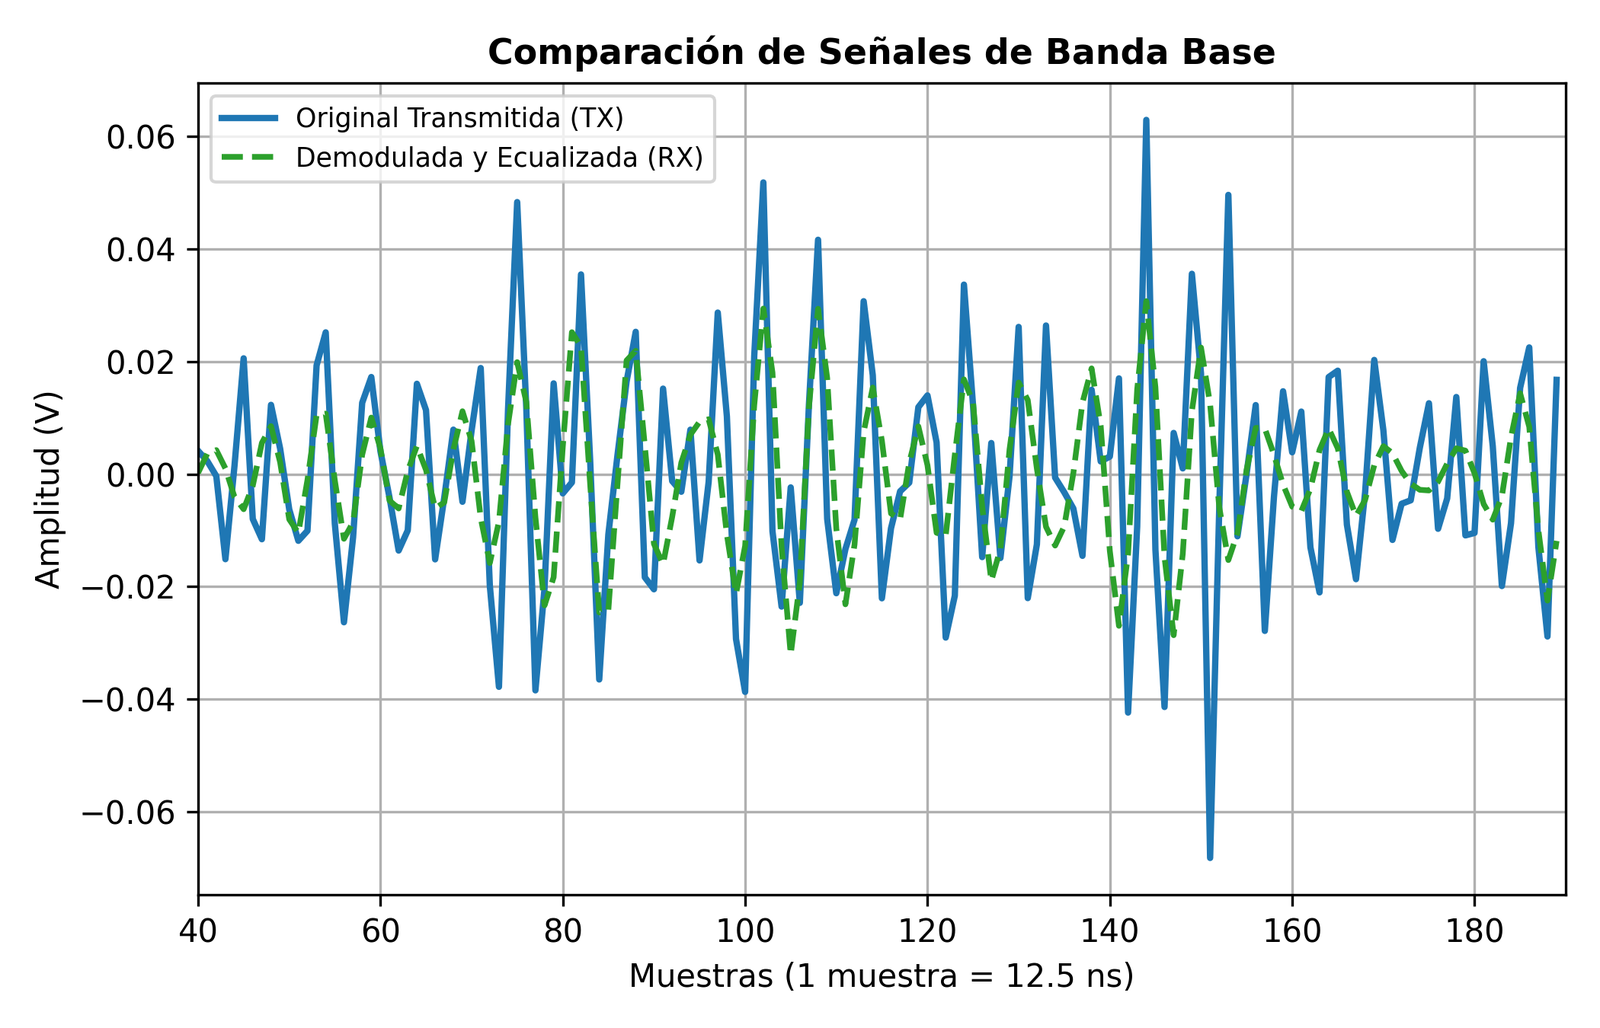
\includegraphics[width=0.75\textwidth]{modulo_comparacion_rx.png}
\caption{Comparación en el dominio del tiempo entre la señal de banda base original transmitida y la señal demodulada y filtrada bajo un enlace ideal sin ruido.}
\label{fig:modulo_comparacion_rx}
\end{figure}

\subsection{GUARD INTERVAL REMOVAL (REMOCIÓN DE INTERVALO DE GUARDA)}
La señal analógica demodulada se corta y organiza en la función \texttt{remove\_guard\_interval()}.

\textbf{Entrada:} señal continua de banda base de longitud $N_{\text{símbolos}} \times (N_{\text{fft}} + N_{\text{CP}})$ muestras. \textbf{Operación:} reorganización en una matriz de $N_{\text{símbolos}}$ filas, descartando los primeros $N_{\text{CP}} = 64$, $128$ ó $256$ muestras por fila según el GI activo. \textbf{Salida:} matriz de $N_{\text{símbolos}} \times 1024$ muestras de datos puros por símbolo OFDM, sin prefijo cíclico, lista para la DFT.

\subsection{DFT/FFT (PROCESAMIENTO DFT)}
El bloque DFT traslada la señal del dominio del tiempo de regreso al dominio de la frecuencia mediante la Transformada Rápida de Fourier (FFT) aplicada a lo largo de las filas de la matriz en la función \texttt{dft\_processing()}, siguiendo la expresión matemática de la ecuación (\ref{eq:dft_theory}) del Capítulo~1.

\textbf{Entrada:} matriz de $N_{\text{símbolos}} \times 1024$ muestras temporales reales. \textbf{Salida:} matriz de $N_{\text{símbolos}} \times 1024$ coeficientes espectrales complejos $Y(k)$ por símbolo, listos para la ecualización FEQ.

\subsection{FEQ / FDE (ECUALIZACIÓN EN FRECUENCIA)}
Antes de extraer los datos, los símbolos complejos en el dominio de la frecuencia se someten a la ecualización FEQ de un solo toque (Ec.~\ref{eq:feq_theory} del Capítulo~1). Esta ecualización se realiza en el script \texttt{test\_phy.py} dividiendo los símbolos complejos de salida entre el factor de ganancia de canal DC de referencia y el filtro analógico estimado.

\textbf{Entrada:} vector espectral $Y(k)$ de 1024 coeficientes. \textbf{Operación:} $\hat{X}(k) = Y(k) / [H_{\text{ref}}(0) \cdot R \cdot H_{\text{filter}}(k)]$. La calibración inicial se realiza en un canal de referencia ideal a distancia fija de $1.0$~m y con un emisor ficticio estándar de semi-ángulo $\theta_{1/2} = 60.0^\circ$ ($m_{\text{ref}} \approx 1$), asegurando que la estimación espectral del filtro sea independiente de la geometría vehicular. \textbf{Salida:} vector de 1024 símbolos complejos ecualizados $\hat{X}(k)$, de los cuales solo se usarán las 234 subportadoras activas. En la Figura~\ref{fig:modulo_constelacion_rx} se presenta el diagrama de constelación resultante tras la ecualización.

\begin{figure}[H]
\centering
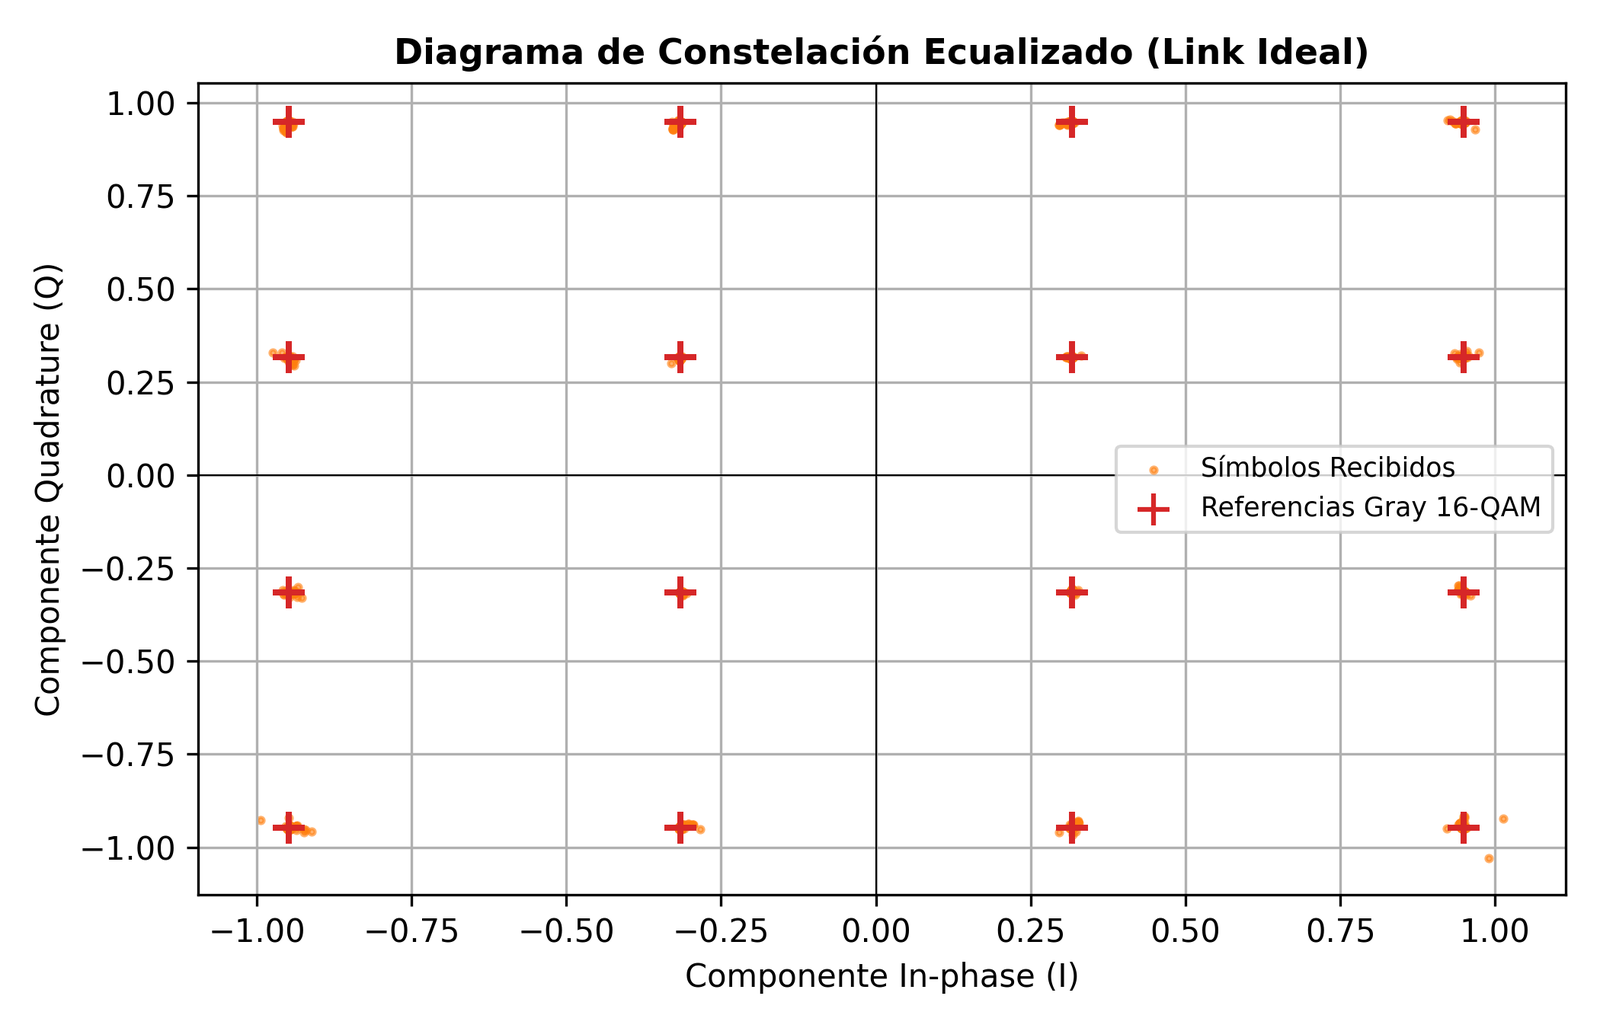
\includegraphics[width=0.75\textwidth]{modulo_constelacion_rx.png}
\caption{Diagrama de constelación ecualizado en el receptor para un esquema 16-QAM bajo un canal óptico ideal libre de interferencias.}
\label{fig:modulo_constelacion_rx}
\end{figure}

\subsection{SUBCARRIER DE-ALLOCATION (EXTRACCIÓN DE SUBPORTADORAS ACTIVAS)}
El bloque \texttt{remove\_hermitian\_symmetry()} extrae los símbolos complejos de datos útiles ecualizados únicamente de las 234 subportadoras positivas activas (índices 139 al 255 y 257 al 373). Las subportadoras de guarda, DC y el espectro simétrico conjugado redundante se descartan por completo.

\textbf{Entrada:} vector de 1024 coeficientes ecualizados. \textbf{Salida:} secuencia lineal de 234 símbolos QAM complejos listos para el demapping de constelación.

\subsection{CONSTELLATION DEMAPPER (DEMAPPING DE CONSTELACIONES)}
La función \texttt{constellation\_demapping()} implementa un demapper de decisión dura para estimar la secuencia de bits. Para BPSK y QPSK se aplican umbrales de decisión sencillos respecto a cero en las componentes en fase (real) y cuadratura (imaginaria). Para constelaciones multinivel complejas (16-QAM, 64-QAM, 256-QAM y 1024-QAM), la función calcula la distancia euclidiana de cada símbolo recibido frente a todos los puntos de referencia normalizados de la constelación Gray teórica, seleccionando el punto con la menor distancia (decisión dura) y recuperando los bits correspondientes.

\textbf{Entrada:} vector de 234 símbolos QAM complejos ecualizados. \textbf{Salida:} vector de bits estimados $\hat{b}$ de longitud $234 \times \log_2(M)$, que pasa al bloque desentrelazador.

\subsection{BLOCK DEINTERLEAVER (DESENTRELAZADOR)}
La secuencia de bits estimada se procesa en la función \texttt{deinterleave()} para revertir el orden de transposición aplicado en el transmisor. Los bits se organizan en una matriz con $n_{\text{cols}} = 16$ (transpuesta de la matriz original) y se reordenan de vuelta a la secuencia secuencial original del flujo de datos, eliminando el relleno (\textit{padding}) residual al final si se requirió en la transmisión.

\textbf{Entrada:} vector de bits estimados entrelazados. \textbf{Salida:} vector de bits desentrelazados en el orden original de transmisión, que pasa al bloque de depunzado y luego al decodificador FEC.

\subsection{FEC DECODER (DECODIFICADOR DE CANAL)}
Finalmente, la secuencia de bits entrelazada pasa al decodificador FEC convolucional en la función \texttt{fec\_decoder()}. Esta función implementa el algoritmo de Viterbi con decisión dura. El algoritmo rastrea las transiciones del codificador convolucional de 4 estados a lo largo de un diagrama de rejilla (\textit{trellis}) calculando de forma iterativa la métrica de camino acumulativa basada en la distancia de Hamming entre los bits recibidos y las salidas válidas de cada transición de estado.

Debido a que se implementa soporte para punzado, el decodificador de Viterbi se modifica para admitir máscaras de borrado (\textit{erasures}). Al procesar los bits, el algoritmo de Viterbi evalúa la máscara \texttt{is\_erasure}. Si detecta que un par de bits corresponde a una posición de borrado (es decir, fue eliminado en el transmisor por el punzado), el decodificador omite sumar la distancia de Hamming en esa transición, manteniendo intacto el trellis métrico y permitiendo la reconstrucción del mensaje original. Al finalizar la secuencia, el algoritmo realiza un proceso de \textit{traceback} desde el estado con la menor métrica acumulada para reconstruir la secuencia de información de entrada original.

\textbf{Entrada:} vector de bits depunzados con máscara de borrados \texttt{is\_erasure}. \textbf{Salida:} vector de bits de información recuperados $\hat{u}$ de longitud $N_{\text{bits}}$. La comparación de este vector con los bits originales $u$ permite calcular la métrica BER (Ec.~\ref{eq:ber}).

\section{ESTRUCTURA DE VALIDACIÓN Y SIMULACIÓN MONTE CARLO}
Para verificar el comportamiento del transmisor y receptor físico LC desarrollado, se implementa una metodología de pruebas funcionales y estadísticas dentro del script de validación \texttt{test\_phy.py}.

\subsection{PROPÓSITO Y ESTRUCTURA DEL SCRIPT DE PRUEBAS (TEST\_PHY.PY)}
El script \texttt{test\_phy.py} constituye el entorno de pruebas automatizadas y validación funcional de la capa física. Está diseñado como un conjunto de rutinas lógicas independientes que aseguran la correctitud de las fases de modulación y demodulación antes de realizar simulaciones bajo ruido solar o atenuaciones. El script se ejecuta directamente desde la consola mediante el intérprete de Python, procesando consecutivamente:
\begin{enumerate}
\item La validación de simetría hermitiana.
\item La transmisión ideal sin ruido de todos los 12 MCS y 3 GIs.
\item El barrido de distancia física y SNR bajo ruido solar de fondo (para GI de 0.8~µs).
\item El barrido analítico de SNR ideal en canal AWGN puro (para GI de 0.8~µs).
\item El barrido comparativo de escenarios climáticos en distancia (para modulación QPSK).
\end{enumerate}

\subsection{VERIFICACIONES FUNCIONALES UNITARIAS}
El script \texttt{test\_phy.py} valida la integridad del transmisor y receptor físico mediante dos rutinas principales:
\begin{enumerate}
\item \textbf{Validación de Simetría Hermitiana:} La función \texttt{test\_hermitian\_symmetry()} genera bits aleatorios, los modula a símbolos complejos, aplica la simetría hermitiana y procesa la IFFT. El script evalúa que la componente imaginaria máxima sea inferior a $10^{-12}$. El cumplimiento del éxito de esta aserción (\texttt{assert}) demuestra que la salida de la IFFT es puramente real y cumple con el principio de transmisión óptica de intensidad.
\item \textbf{Validación de Canal Ideal:} La función \texttt{test\_ideal\_channel()} interconecta el transmisor y el receptor en un canal óptico de 1.0~metros sin añadir ruido aleatorio ($\sigma^2_{\text{total}} = 0.0$). El script comprueba la ausencia de discrepancias binarias tras la decodificación, validando que las fases de codificación, punzado, modulación, filtrado, sincronización, demodulación, depunzado y decodificación de Viterbi funcionen de forma correcta y simétrica para todos los 12 MCS y 3 GIs definidos.
\end{enumerate}

\subsection{SIMULACIÓN DE MONTE CARLO Y PRECISIÓN ESTADÍSTICA}
La evaluación del rendimiento de la comunicación bajo escenarios de ruido aleatorio en exteriores se realiza mediante el método de Monte Carlo. Debido a la naturaleza estocástica del ruido de disparo solar y el ruido térmico, no es suficiente evaluar una única transmisión corta para caracterizar el enlace. La simulación Monte Carlo repite el proceso de transmisión bajo la generación independiente de bits de información aleatorios para cada simulación, añade ruido aleatorio (de disparo solar y térmico) en el dominio óptico equivalente a través de la función del canal y cuenta de forma acumulativa los errores de bit resultantes en el extremo receptor.

La Tasa de Error de Bit (BER) se calcula de forma estadística dividiendo los bits erróneos decodificados a la salida del algoritmo de Viterbi entre la longitud total de la secuencia útil de bits de información, de acuerdo con la Ec.~\ref{eq:ber} del Capítulo~1. A partir de este valor, la velocidad de transmisión efectiva (\textit{Throughput}) en Mbps se estima deduciendo los bits erróneos de la tasa bruta nominal ($R_{\text{raw}}$), siguiendo la Ec.~\ref{eq:throughput} del Capítulo~1. 

La velocidad física bruta $R_{\text{raw}}$ se determina según los parámetros de subportadoras de datos activas ($N_{\text{active}} = 234$), el orden de la modulación ($M$), la tasa de codificación ($R_c$) y la duración del símbolo OFDM ($T_{\text{symbol}}$) definidos por el estándar e implementados en el simulador.


Para garantizar la flexibilidad computacional e independencia estadística, el script \texttt{test\_phy.py} incorpora una constante global de control denominada \texttt{MONTE\_CARLO\_RUNS}. A partir de esta constante, se configuran de manera proporcional las variables independientes de bits para cada simulación: $N_{\text{BITS\_SOLAR}} = \text{MONTE\_CARLO\_RUNS}$ para el barrido físico, $N_{\text{BITS\_IDEAL}} = \text{MONTE\_CARLO\_RUNS}$ para el barrido analítico ideal y $N_{\text{BITS\_ESCENARIOS}} = \text{MONTE\_CARLO\_RUNS}$ para los escenarios meteorológicos. 

Para las simulaciones finales de caracterización física presentadas en este trabajo, se configuró la constante en \texttt{MONTE\_CARLO\_RUNS = 100000}. Esta cantidad de bits de prueba de información proporciona una precisión estadística suficiente para registrar tasas de error de bit de hasta $10^{-5}$ con un intervalo de confianza estrecho. De igual manera, se utiliza una semilla de aleatoriedad fija mediante \texttt{np.random.seed(123)} para asegurar que los bits generados en cada ejecución sean idénticos, permitiendo comparar los MCS bajo las mismas condiciones y garantizar la repetibilidad de las pruebas.

\subsection{CONFIGURACIÓN CENTRALIZADA DEL SIMULADOR}
Para garantizar la coherencia física y la facilidad de mantenimiento de las simulaciones de la capa física, el simulador del transmisor y receptor VLC/V2I centraliza sus parámetros de diseño (tanto del transmisor y receptor OFDM como de la geometría del canal óptico) en un único archivo de configuración denominado \texttt{config\_entorno.py}. Este archivo es importado por todos los módulos del simulador (\texttt{main.py}, \texttt{test\_phy.py} y \texttt{test\_phy\_grid.py}). La estructura de directorios de este simulador y la guía paso a paso de su instalación se detallan en el Anexo \ref{anexo:manual_simulador} y Anexo \ref{anexo:estructura_archivos_simulador}.

Los reportes gráficos correspondientes a la validación cualitativa paso a paso del procesamiento de las señales y los diagramas de constelación del transmisor y receptor se han consolidado al inicio del Capítulo 3 (sección de Resultados y Discusión) para mantener agrupados todos los análisis experimentales y cualitativos antes del barrido masivo de rendimiento.
